\documentclass[10pt]{article}
\usepackage{mathpaper}
\begin{document}
\section*{\centering 第二十二章~~~二次函数}
\centerline{时间:2小时 \ \ \ \ 满分:120分}
\section*{\normalsize 一、选择题(每小题3分,共30分)}
\begin{enumerate}\setcounter{enumi}{0}
    \item %1
    \item %2
    \item %3
    \item %4
    \item %5
    \item %6
    \item %7
    \item %8
    \item %9
    \item 如图,在平行四边形$ABCD$中,$BC=2AB=20$,$B$、$F$、$E$三点共线,且$\angle ABC=60^{\circ}$。连$AF$、$AE$、$CE$,若$AE=EF$,$\angle DAE+\angle CBF=60^{\circ}$,且$AF=6$,则$\Delta BEC$的面积为(~~~~~~~)。
    \onp{$16\sqrt{3}$}{$68\sqrt{3}$}{$32\sqrt{3}$}{$34\sqrt{3}$}
\end{enumerate}
\begin{figure}[htb]
    \centering
    \subfigure[(第10题)]{
    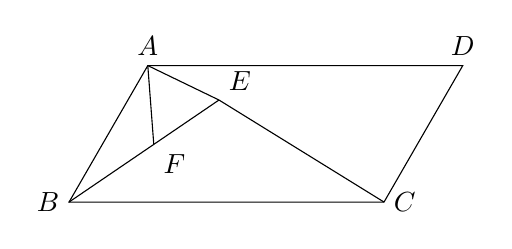
\begin{tikzpicture}[scale=0.4]
        \coordinate[label=above:{$A$}] (A) at (2.5,4.33333);
        \coordinate[label=left:{$B$}] (B) at (0,0);
        \coordinate[label=above:{$D$}] (D) at (12.5,4.33333);
        \coordinate[label=right:{$C$}] (C) at (10,0);
        \coordinate[label=above right:{$E$}] (E) at (4.76,3.24);
        \coordinate[label=below right:{$F$}] (F) at (2.69,1.83);
        \draw (A)--(B)--(C)--(D)--cycle;
        \draw (A)--(F);
        \draw (A)--(E);
        \draw (C)--(E);
        \draw (B)--(E);
    \end{tikzpicture}}
\end{figure}
\section*{\normalsize 二、填空题(每小题3分,共18分)}
\begin{enumerate}\setcounter{enumi}{10}
    \item %11
    \item %12
    \item %13
    \item %14
    \item %15
    \item 若关于$x$的一元二次方程$x^2+(k-2)x-k^2-1=0$有一根大于$k$,另一根小于$k$,则$k$的取值范围是\complitingline{}。
\end{enumerate}
\section*{\normalsize 三、解答题(共8题、72分,每小题应写出文字说明、解答过程或演算步骤)}
\begin{enumerate}\setcounter{enumi}{16}
    \item %17
    \begin{compactenum}[(1)]
        \item %17.1
        \item %17.2
    \end{compactenum}
    \item %18
    \begin{compactenum}[(1)]
        \item %18.1
        \item %18.2
    \end{compactenum}
    \item %19
    \begin{compactenum}[(1)]
        \item %19.1
        \item %19.2
    \end{compactenum}
    \item
    \begin{compactenum}[(1)]
        \item %20.1
        \item %20.2
    \end{compactenum}
    \item %21
    \begin{compactenum}[(1)]
        \item %21.1
        \item %21.2
    \end{compactenum}
    \item %22
    \begin{compactenum}[(1)]
        \item %22.1
        \item %22.2
        \item %22.3
    \end{compactenum}
    \item %23
    \begin{compactenum}[(1)]
        \item %23.1
        \item %23.2
        \item %23.3
    \end{compactenum}
    \item %24
    \begin{compactenum}[(1)]
        \item %24.1
        \item %24.2
        \item %24.3
    \end{compactenum}
\end{enumerate}
\end{document}